\section{Floating Point Model}\label{sec:float}

The first model we have to write is a floating point version of \cordic{}
algorithm as we can see in \lstref{lst:cordicfloatmatlab}.

\lstinputlisting[language=matlab, label={lst:cordicfloatmatlab},
caption={CORDIC Floating Point Model in Matlab
(\code{cordic\_vectoring\_float.m}).}]{matlab/float/cordic_vectoring_float.m}

From this model we can obtain a measure of the algorithmic error, comparing the
output of this algorithm, produced with a test input dataset\footnote{The test
input dataset is composed by points lying on circumferences with different
radius}, and compared to the radius and phase computed in ``traditional'' way.

The result is that both on phase and radius the error after 14 iterations is in
the order of \(10^{-9}\) for the radius (as shown in
\figref{fig:floaterrorradius}) and \(10^{-4}\) for the phase (as shown in
\figref{fig:floaterrorphase}). The resulting \emph{Mean Square Errors} and
\emph{Max Errors} are shown in~\eqref{eq:errorfloat}.

\begin{equation}\label{eq:errorfloat}
	\begin{array}{rl}
		MSE_r &= 2.8876\times10^{-18}\\
		MSE_p &= 4.2575\times10^{-9}\\
		MaxError_r &= 6.3350\times10^{-9}\\
		MaxError_p &= 1.1865\times10^{-4}
	\end{array}
\end{equation}

\begin{figure}[htb]
	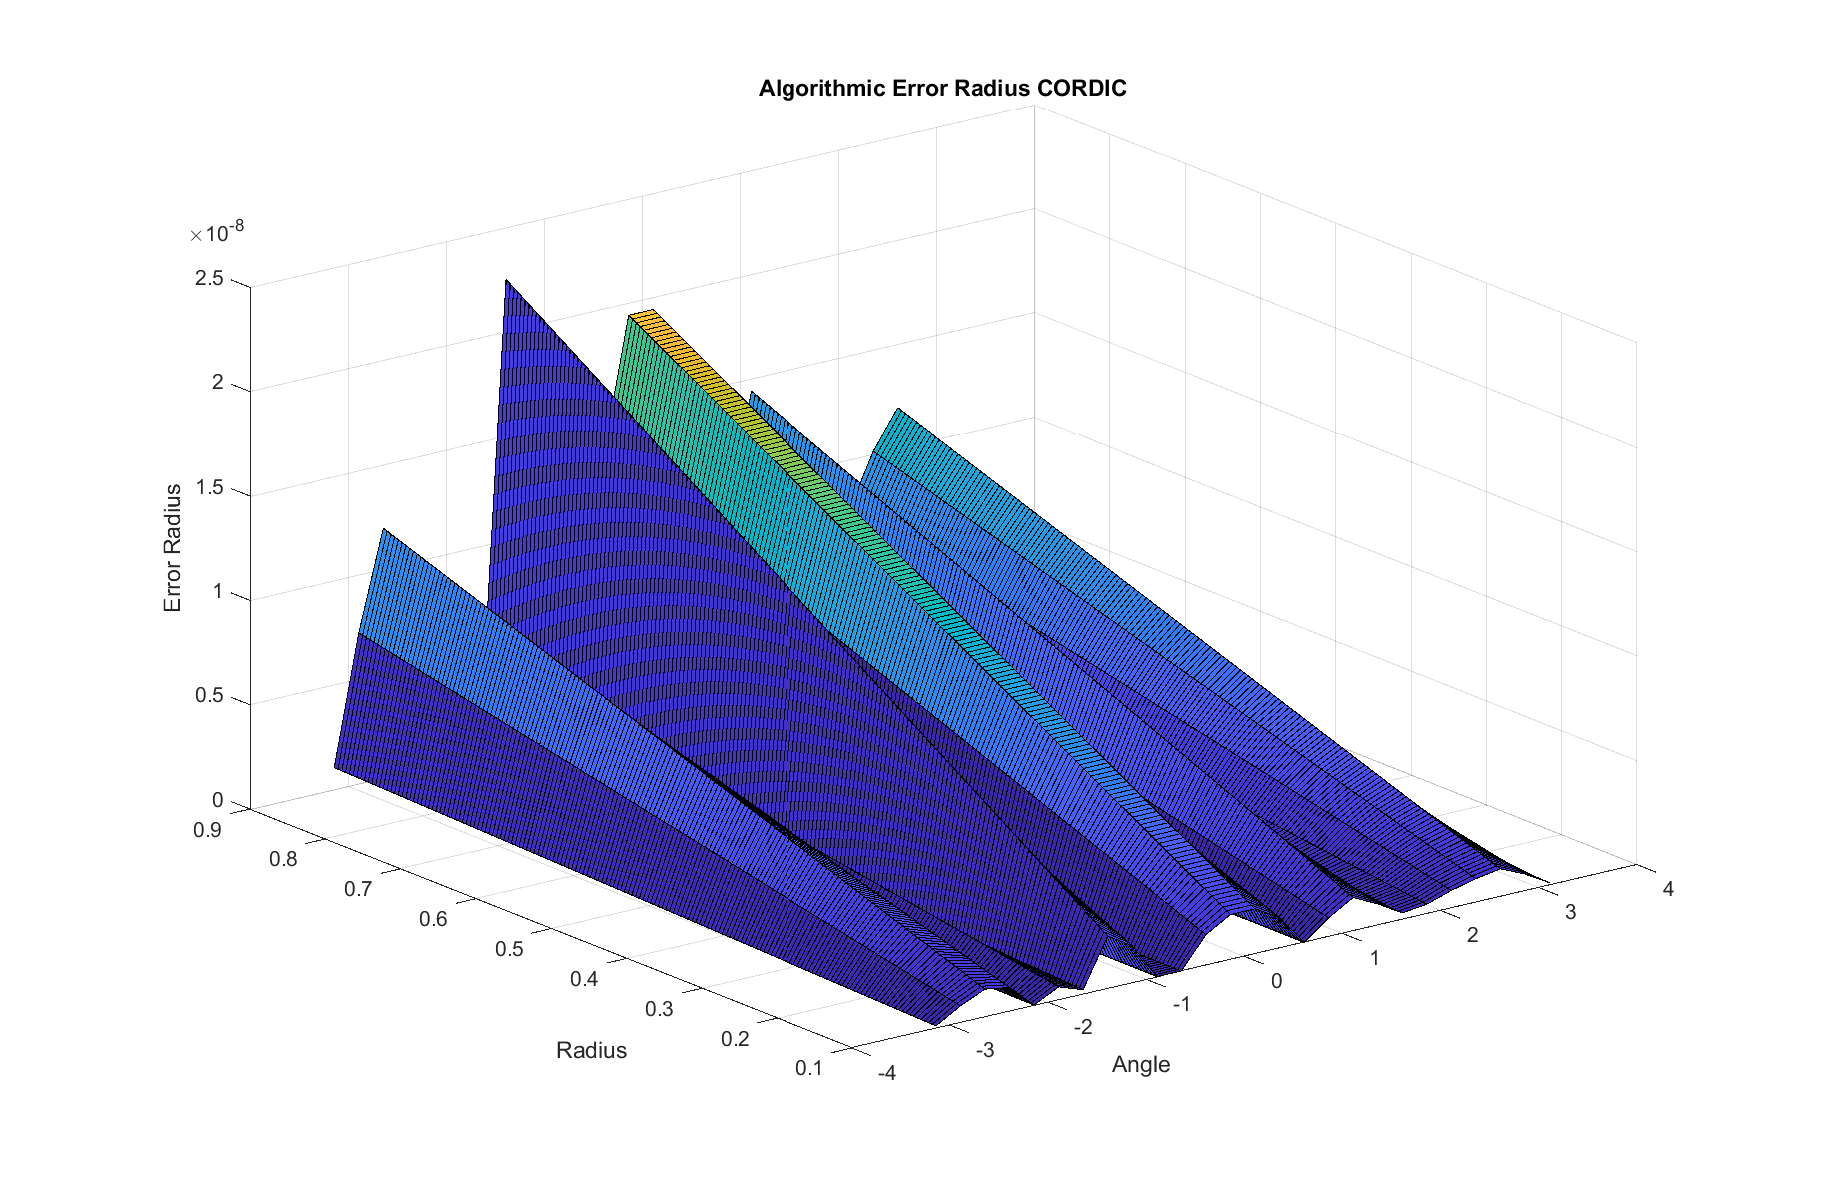
\includegraphics[width=\textwidth]{alg_error_radius}
	\caption{Algorithmic Error Radius.}\label{fig:floaterrorradius}
\end{figure}
\begin{figure}[htb]
	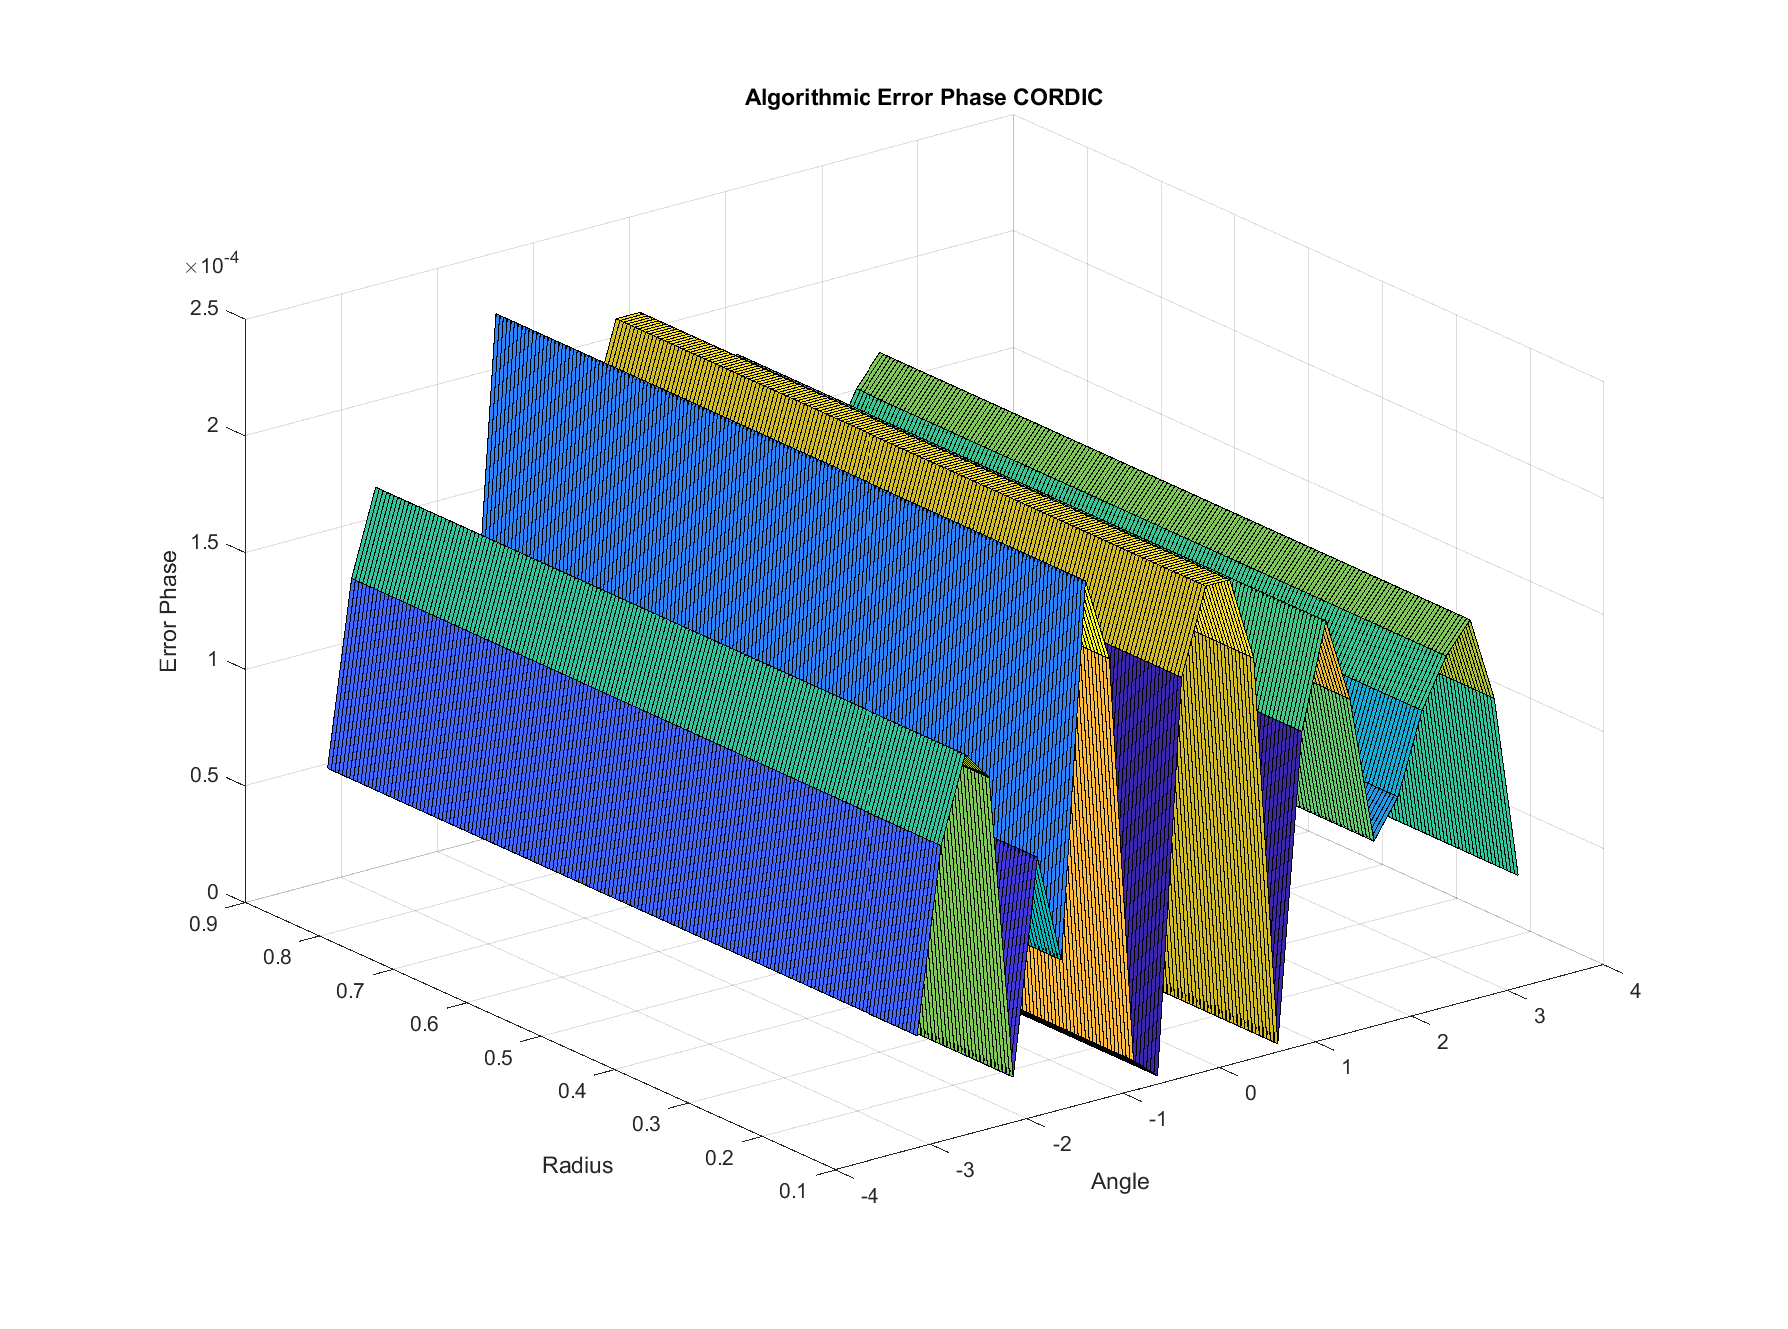
\includegraphics[width=\textwidth]{alg_error_phase}
	\caption{Algorithmic Error Phase.}\label{fig:floaterrorphase}
\end{figure}
